In the following chapter we will try to summarise the results we got from our ambient occlusion solution as well as compare the two implemented sampling methods and their efficiency with regard to the number of used samples.
\section{Comparison of ambient occlusion results}
This section contains comparison of results using rejection sampling (described in \autoref{sec:rejection_sampling}) to the use of cosine weighted hemisphere sampling (\autoref{sec:cosine_weighted}). The renders were run with 100, 200 and 300 sample rays and the results can be seen in \autoref{fig:AO_renders}.

\begin{figure}[h!]
	\centering
	\subfloat[100 samples, rejection sampling]{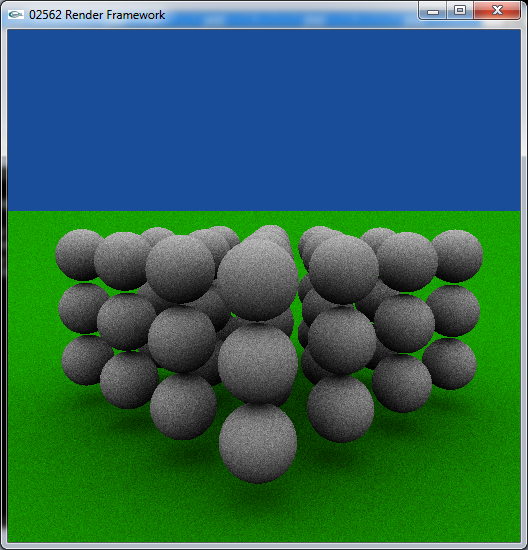
\includegraphics[width=.4\textwidth]{Results/rejection100.png}}
    	\subfloat[100 samples, cosine weighted sampling]{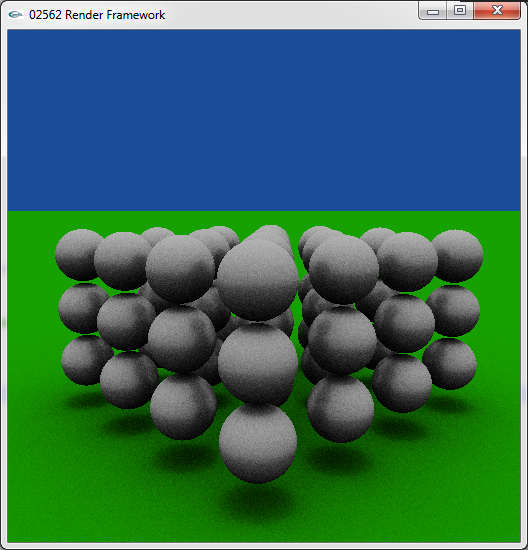
\includegraphics[width=.4\textwidth]{Results/cosine100.png}}\\
    	\subfloat[200 samples, rejection sampling]{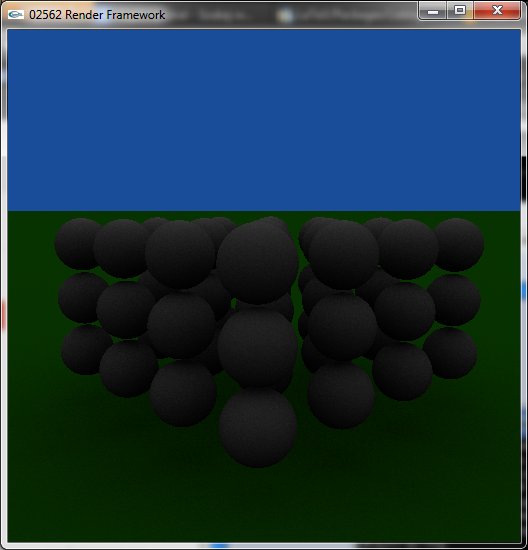
\includegraphics[width=.4\textwidth]{Results/rejection200.png}}
    	\subfloat[200 samples, cosine weighted sampling]{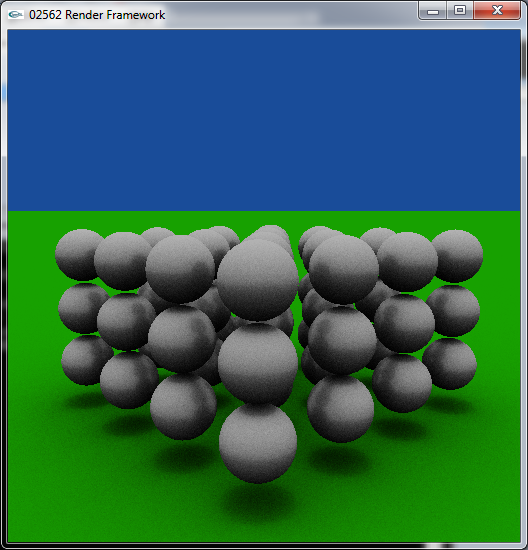
\includegraphics[width=.4\textwidth]{Results/cosine200.png}}\\
	\subfloat[300 samples, rejection sampling]{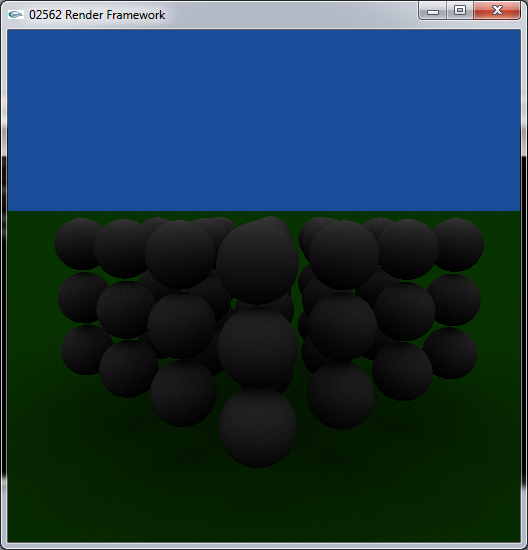
\includegraphics[width=.4\textwidth]{Results/rejection300.png}}
    	\subfloat[300 samples, cosine weighted sampling]{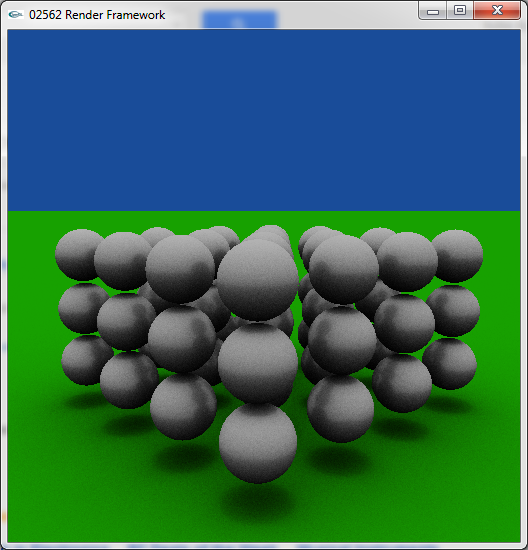
\includegraphics[width=.4\textwidth]{Results/cosine300.png}}\\
	\caption{Comparison of sampling methods if different number of samples}
	\label{fig:AO_renders}
\end{figure}